%%%%%%%%%%%%%%%%%%%%%%%%%%%%%%%%%%%%%%%%%%%%%%%%%%%%%%%%%%%%%%%%%%%%%%%%
% Plantilla TFG/TFM
% Escuela Politécnica Superior de la Universidad de Alicante
% Realizado por: Jose Manuel Requena Plens
% Contacto: info@jmrplens.com / Telegram:@jmrplens
%%%%%%%%%%%%%%%%%%%%%%%%%%%%%%%%%%%%%%%%%%%%%%%%%%%%%%%%%%%%%%%%%%%%%%%%

\chapter{Introducción}

La gestión y recuperación eficiente de la información digital se ha convertido en un desafío cotidiano en la era de la sobrecarga informativa. Los volúmenes de datos personales y profesionales que almacenamos en nuestros dispositivos crecen exponencialmente, mientras que las herramientas tradicionales de búsqueda a menudo resultan insuficientes para localizar archivos específicos de manera rápida y precisa. Este proyecto se adentra en esta problemática, proponiendo una solución innovadora basada en los avances recientes en \gls{ia} y sistemas de Generación Aumentada por Recuperación (\gls{rag}).

\section{Panorama Actual: Desafíos en la Recuperación de Información}
Los métodos convencionales para la organización y búsqueda de archivos digitales se basan en gran medida en metadatos explícitos, como nombres de archivo, fechas o etiquetas manuales. Sin embargo, estas aproximaciones tienen limitaciones significativas:
\begin{itemize}
\item  \textbf{Insuficiencia de los metadatos tradicionales:} A menudo, los metadatos son inexistentes, incompletos o no capturan la semántica real del contenido del archivo (especialmente en el caso de imágenes, vídeos o audios).
\item  \textbf{Falta de precisión en las búsquedas:} Las búsquedas basadas en palabras clave pueden ser ambiguas y no siempre interpretan correctamente la intención del usuario, llevando a resultados irrelevantes o a la omisión de la información que el usuario desea encontrar.
\item  \textbf{Desafíos técnicos y éticos en \gls{ia}:} Si bien la \gls{ia} ofrece nuevas vías, también enfrenta retos. Los modelos pueden carecer de la precisión necesaria para ciertas tareas o, en el caso de modelos generativos, incurrir en ``alucinaciones'' (generar información incorrecta pero plausible). Además, el propio entrenamiento del modelo puede afectar a la interpretación sobre el archivo que se quiere describir, generando resultados no equitativos o discriminatorios, lo que plantea también importantes consideraciones éticas.
\item \textbf{Riesgos de seguridad y privacidad de los datos:} La externalización del almacenamiento a la nube y el uso de \gls{ia} para la catalogación y el análisis de ficheros introducen nuevas formas de ataque y preocupaciones sobre la seguridad y privacidad. Estos sistemas pueden ser vulnerables a accesos no autorizados, fugas de datos o ciberataques, tanto en la infraestructura cloud como en los propios modelos de \gls{ia}. La información sensible contenida en los archivos, o incluso los metadatos enriquecidos generados por la \gls{ia}, podrían quedar expuestos, ser alterados o perderse. Esto es especialmente crítico cuando se manejan datos confidenciales o personales, donde una brecha de seguridad no solo implica la pérdida de información valiosa, sino también posibles consecuencias legales, financieras y reputacionales significativas.
\end{itemize}
Este contexto muestra la necesidad de sistemas más inteligentes y contextuales capaces de comprender el contenido de los archivos de forma más profunda, más allá de sus metadatos superficiales, y que al mismo tiempo garanticen la integridad y confidencialidad de la información.

\section{Avances Tecnológicos Fundamentales}
Para abordar los desafíos mencionados, este proyecto se apoya en los desarrollos más recientes en el campo de la Inteligencia Artificial, particularmente en las siguientes áreas:

\subsection{Inteligencia Artificial Multimodal: Convergencia de Lenguaje y Visión}
La Inteligencia Artificial ha experimentado avances exponenciales, especialmente con el auge del \gls{pln} y la Visión Artificial. La multimodalidad representa la capacidad de los sistemas de \gls{ia} para procesar, comprender y generar información a partir de múltiples tipos de datos (o ``modalidades'') simultáneamente, como texto, imágenes, audio y vídeo.
\begin{itemize}
    \item Procesamiento del Lenguaje Natural (\gls{pln}): Permite a las máquinas comprender, interpretar y generar lenguaje humano. Los Grandes Modelos de Lenguaje (\gls{llm}), como \gls{gpt} (Generative Pre-trained Transformer) y sus variantes, han revolucionado este campo, demostrando una capacidad asombrosa para entender el contexto, generar texto coherente e incluso razonar sobre la información proporcionada.
    \item Visión Artificial: Es la disciplina que permite a las máquinas ``ver'' e interpretar el contenido de imágenes y vídeos. Implica tareas como la detección de objetos, el reconocimiento facial, la segmentación de imágenes y la generación de descripciones visuales.
    \item Modelos Multimodales (ej. \gls{clip})\footnote{Más información sobre \gls{clip} de OpenAI disponible en: \url{https://openai.com/es-ES/index/clip/}}: Modelos como \gls{clip} (Contrastive Language-Image Pre-training) de OpenAI son un ejemplo paradigmático de esta convergencia. \gls{clip} aprende representaciones visuales a partir de descripciones en lenguaje natural, permitiendo realizar búsquedas de imágenes mediante consultas textuales con una alta comprensión semántica, o viceversa. Funciona entrenando un codificador de imágenes y un codificador de texto para predecir qué imágenes se emparejan con qué textos en un gran conjunto de datos.
\end{itemize}

\subsection{Optimización de Modelos: Cuantización y Modelos Ligeros}
Para la aplicación práctica de estos modelos, especialmente en entornos con recursos limitados (como dispositivos personales), es crucial considerar su eficiencia.
\begin{itemize}
    \item Modelos Cuantizados: La cuantización es un proceso que reduce la precisión numérica de los pesos y activaciones de un modelo de red neuronal (por ejemplo, de punto flotante de 32 bits a enteros de 8 bits). Esto disminuye significativamente el tamaño del modelo y acelera la inferencia, con una pérdida de precisión a menudo mínima.
    \item Modelos Ligeros (Lightweight Models): Son arquitecturas de redes neuronales diseñadas específicamente para ser computacionalmente eficientes y tener un tamaño reducido, facilitando su despliegue en dispositivos móviles o embebidos sin sacrificar excesivamente el rendimiento.
\end{itemize}

\subsection{Sistemas de Generación Aumentada por Recuperación (\gls{rag})}
La Generación Aumentada por Recuperación (\gls{rag}) es una técnica que mejora el rendimiento de los \gls{llm} al conectarlos con fuentes de conocimiento externas. En lugar de depender únicamente de la información (potencialmente desactualizada o incompleta) aprendida durante su entrenamiento, un sistema \gls{rag} funciona en dos fases:
\begin{enumerate}
    \item Recuperación (Retrieval): Dada una consulta del usuario, el sistema primero busca y recupera fragmentos de información relevante de una base de datos, un conjunto de documentos o un corpus de conocimiento. Esta base de datos puede estar compuesta por embeddings (representaciones vectoriales densas) del contenido de los archivos.
    \item Generación (Generation): La información recuperada se proporciona como contexto adicional al \gls{llm} junto con la consulta original. El \gls{llm} utiliza este contexto enriquecido para generar una respuesta más precisa, relevante y fundamentada.
\end{enumerate}
Los sistemas \gls{rag} ofrecen ventajas significativas, como la reducción de alucinaciones, la capacidad de citar fuentes del contexto dado y la facilidad para actualizar la base de conocimiento sin necesidad de reentrenar el \gls{llm} completo. Si bien existen diversas arquitecturas \gls{rag} (ej. generando consultas SQL, incorporando texto directamente al prompt, o utilizando embeddings), el enfoque basado en embeddings suele ofrecer un buen equilibrio entre eficiencia y calidad de los resultados, aunque presenta desafíos como la gestión de la ventana de contexto del \gls{llm}, punto crucial a tener en cuenta si se utilizan sobre dispositivos personales.

\bigskip % Añade un poco de espacio vertical antes de la figura
\begin{figure}[H] % [H] intenta forzar la posición "aquí"
    \centering % Centra la imagen en la página
    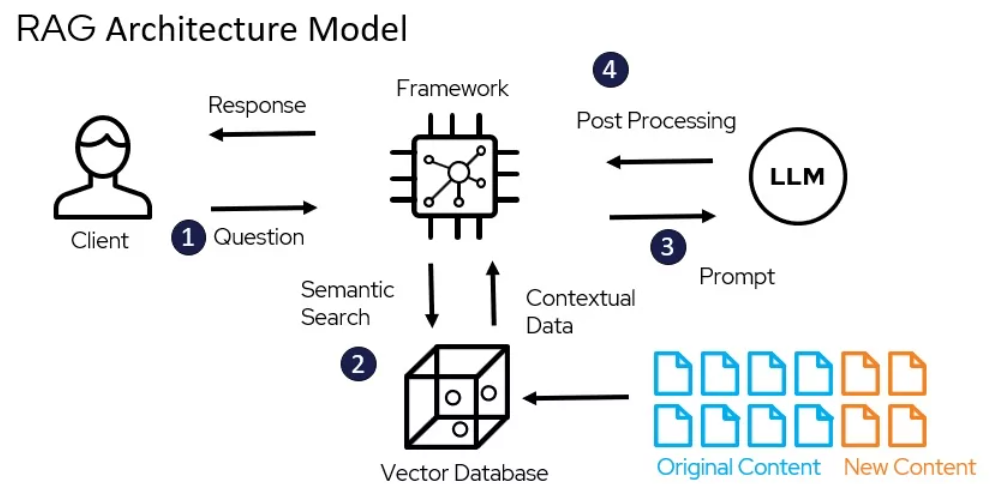
\includegraphics[width=0.8\textwidth]{archivos/RAG_scheme.png} % Ajusta el ancho como necesites
    \caption[Esquema de un sistema RAG]{Esquema visual del funcionamiento de un sistema RAG, mostrando el flujo desde la consulta del usuario, pasando por la recuperación de información relevante, hasta la generación de la respuesta final por el LLM.}
    \label{fig:rag_scheme} % Etiqueta para referenciar la figura en el texto
\end{figure}
\bigskip % Añade un poco de espacio vertical después de la figura

\subsection{Justificación del Proyecto}
Este \gls{tfg} busca abordar la necesidad de obtener información de manera rápida, sencilla y muy precisa desarrollando un sistema inteligente de búsqueda de archivos que permita a los usuarios encontrar información utilizando consultas en lenguaje natural, trascendiendo las limitaciones de las búsquedas basadas en metadatos tradicionales. La aplicación de modelos multimodales permitirá indexar el contenido semántico de diversos tipos de ficheros, y la arquitectura \gls{rag} proporcionará un marco robusto para recuperar la información más relevante y presentarla de forma útil al usuario.